\documentclass[preprint,12pt]{article}

\usepackage{algorithmic}
\usepackage{algorithm}
\usepackage{enumerate}
\usepackage{enumitem}
\usepackage{graphics}
\usepackage{graphicx}
\usepackage{geometry}
\usepackage{amsmath}
\usepackage{wrapfig}
\usepackage{subfig}
\usepackage{framed}
\usepackage{color}
\usepackage{soul}
\usepackage{bm}

\usepackage{natbib}
\usepackage{multirow}
\usepackage[T1]{fontenc}
\usepackage[latin9]{inputenc}
%\usepackage{units}
\usepackage{esint}
\geometry{legalpaper,  margin=1in}

\newcommand{\CM}[2][green]{ {\sethlcolor{#1} \hl{#2}} }
\newcommand{\KB}[2][cyan]{ {\sethlcolor{#1} \hl{#2}} }
%THIS IS TO PUT ALL FLOATS AT THE END OF THE DOC SO THEY CAN BE SPLIT INTO A SEPARATE FILE
%%\usepackage{endfloat}
%\makeatother

%\usepackage{babel}

\begin{document}
\title{A comparison of the effects of Redstricting Algorithms on Partisan Gerrymandering}

\author{Kevin Baas}

\maketitle

\begin{abstract}
We use federal congressional districts for all 50 states, for redistricing cycle 2001-2011, and 2011-2021.  We then use Auto-Redistrict to generate alternative congressional districts for all 50 states, using a number of different algorithms to generate the districts, including compactness-only, fairness optimized, and multi-member districts.

We then use an Empirical Bayesian probability model that we outlined and validated in a previous paper, combined with ward-resolution data from three consecuitive presidential elections, to compute likelihood curves for both popular vote and seats won, for all of these redistricting algorithms, and compare the results.

Using all 50 states gives a broad mix of demographics and geography, providing an informative and diverse set of samples, and allowing us to rule out effects that are idiosyncratic idiosyncratic to particular states, such as urban vs. rural states, or swing states vs. safe states.

We find that the current official method for redistricting (hand-drawn) produces the least representative outcomes of all those considered.  Conversely, heuristic optimization produces the most representative outcomes.  We also find that multi-member districts produce far more representative outcomes than their single-member counterparts.

In addition to suggesting a way forward for creating more representative electoral districts, the methods we outline in our paper provide a way to do a comprehensive analysis of the partisan impact of any proposed redistricting plan.  Because it is a Bayesian model, it produces complete likelihood curves, as opposed to a single point estimate.  This gives both legislative and judicial reviewers a more complete picture of the impact of the plan, including a picture of the durability of the effects.

Keywords: Redistricting, gerrymander, modeling

\end{abstract}

\clearpage

\section{Visualizing the outcomes}

Using a Bayesian model enables us to calculate complete likelihood curves, as opposed to just point estimates, for any quantity that we can formally describe.  These likelihood curves can be generated by sampling the posterior predictive distribution, and then applying the formula for the measured quantity to the samples.

In an effort to give a comprehensive visual representation of these likelihoods, we graph a 3-dimensional chart showing on one axis a potential popular vote fraction, on another axis a potential seat count, and on the third, the probability of that combination.  The function being graphed is z = p( vote percent, seat count). "z" is represented by color saturation (darkness).  In this way, the chart resembles a "heat map".

\section{What the U.S. House would be like under alternative districting algorithms}

We used presidential election data from 2004, 2008, and 2012 elections, at voting ward resolution, from Stephen Wolf of DailyKo's Google drive.  We then used AutoRedistrict to design heuristically optimized districts for all 50 states, for single member and multi-member proportional districts, both for the current 435 seat count and a theoretically expanded seat count of 593.  To this we added the current actual districts, the previous census cycle's districts, and compactness-optimized districts created using BDistricting.   We then used AutoRedistrict to combine the district shapes with the ward-resolution election vote counts, and export district-resolution election vote counts, for all 3 elections.

We then used our empirical Beta model to compute likelihoods curves for each of these redistricting methods. 

These methods can also be applied at state and local levels (e.g. state legislative, city council), and on different types of districts (e.g. police districts, voting wards)

\begin{figure}[htb!]
    \begin{center}
        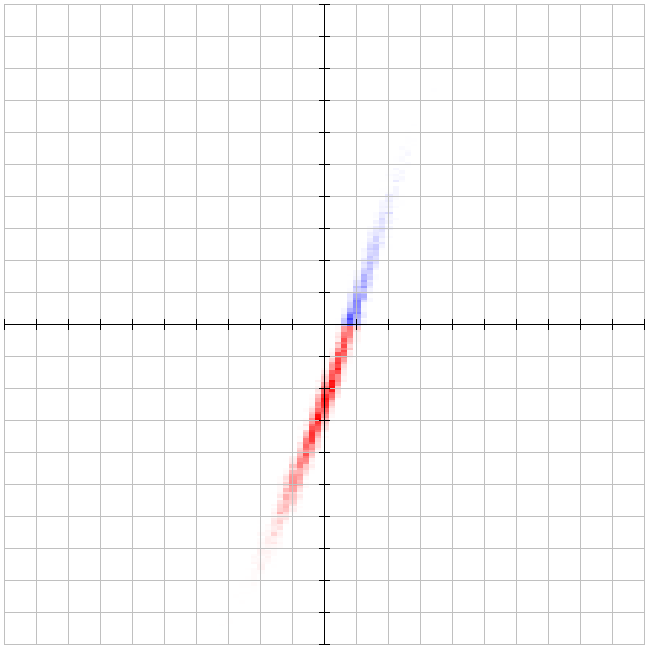
\includegraphics[scale=0.5]{Figures/original_method/2010_ush.png}
        \caption{2010 U.S. House districts, seats-votes likelhoods}\label{fig:2010_ush}
    \end{center}
\end{figure}
\begin{figure}[htb!]
    \begin{center}
        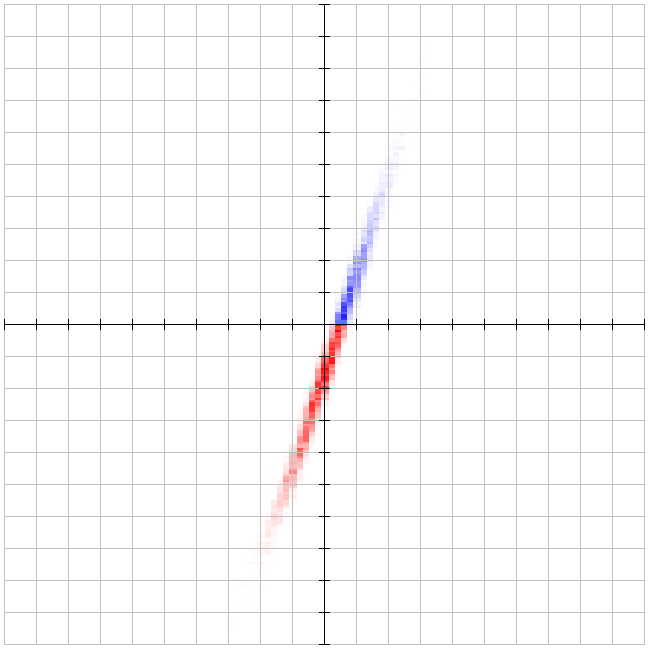
\includegraphics[scale=0.5]{Figures/original_method/2000_ush.png}
        \caption{2000 U.S. House districts, seats-votes likelhoods}\label{fig:2000_ush}
    \end{center}
\end{figure}
\begin{figure}[htb!]
    \begin{center}
        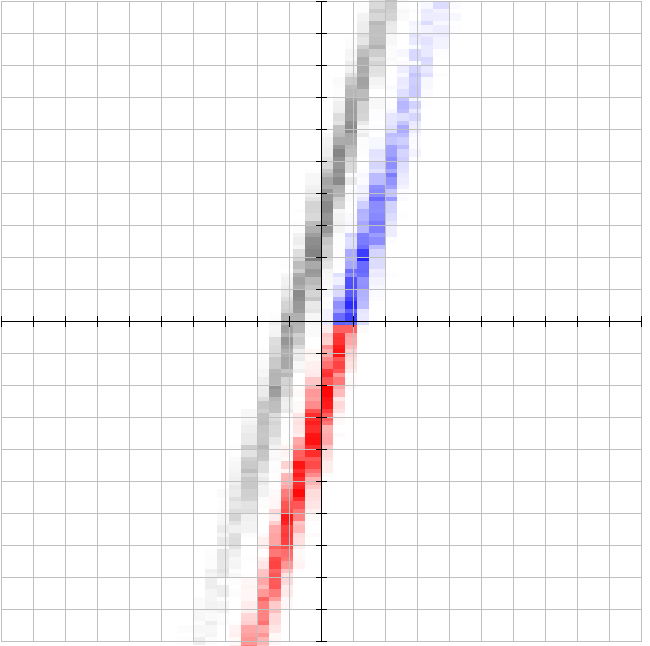
\includegraphics[scale=0.5]{Figures/original_method/BD__ush.png}
        \caption{Compactness optimized U.S. House districts, seats-votes likelhoods}\label{fig:BD_ush}
    \end{center}
\end{figure}
\begin{figure}[htb!]
    \begin{center}
        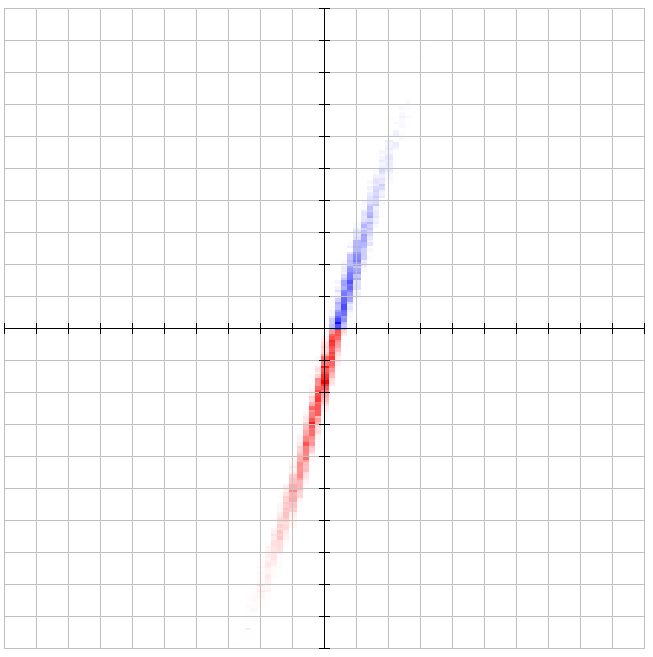
\includegraphics[scale=0.5]{Figures/original_method/SM__ush.png}
        \caption{Multi-objective optimized U.S. House districts, seats-votes likelhioods}\label{fig:SM_ush}
    \end{center}
\end{figure}
\begin{figure}[htb!]
    \begin{center}
        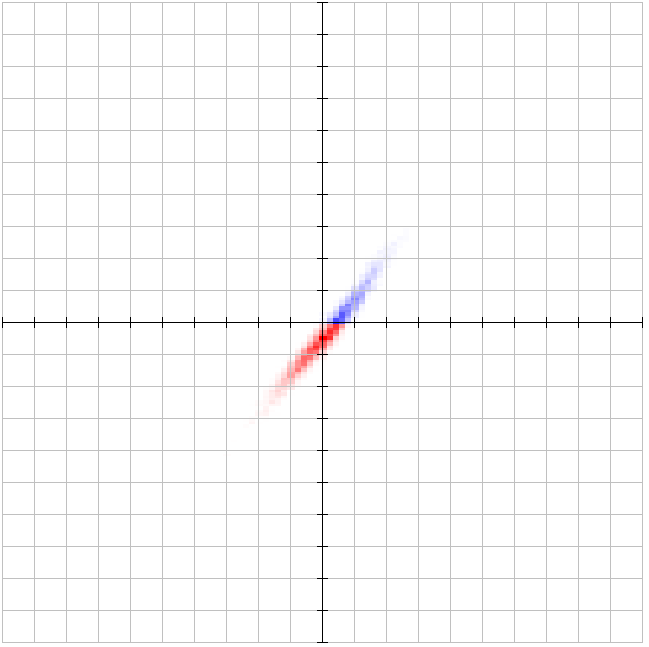
\includegraphics[scale=0.5]{Figures/original_method/FV_droop_ush.png}
        \caption{Multi-member proportional U.S. House districts, seats-votes likelhioods}\label{fig:FV_ush}
    \end{center}
\end{figure}

Our results indicate that in the 2010 redistricting cycle, Republicans systematically gerrymandered the U.S. House, giving Democratic voters a large structural disadvantage. The popular vote would have to favor Democrats by more than an 8 percent margin, just to give them a majority of seats.  This contrasts sharply with what seats-votes likelihoods would be like if elections were still held under the districts from the 2000-cycle redistricting.  If the partisan gerrymandering in 2010 did not occur, Democratic voters would only have to win the popular vote by a little over 5 percent margin in order to get half of the U.S. house seats.

If instead all states in the country used an algorithm to optimize compactness of districts, the result would be about the same.  This suggests that most of the gerrymandering in the 2000-cycle was accidental; that it was due to political self-sorting, as opposed to deliberate gerrymandering.  If instead all states in the country used an alogirhtm that also minimized seats-votes curve asymmetry, the amount of partisan gerrymandering would be further reduced, and Democrats would only have to win the popular vote by a 3 percent margin in order to win the majority of seats.

Finally, using multi-member proportional districts appears to further reduce partisan gerrymandering, in addition to making the seat allocations more proportional.  Our nation-wide statistical analysis of alternative redistricting algorithms suggests that, when it comes to representation, the voting and tallying system is far more important than the redistricting algoorithm.  In other words, if the goal is to eliminate gerrymandering and make elections more responsive, then instead of focusing on how changes to the redistricting process can reduce or eliminate gerrymandering, we should be focused on a fundamental overhaul on how congressional seats are assigned.

We were surprised to find that even with multi-member proportional districts, there remains a small amount of partisan asymmetry in favor of Republicans.
A possible explanation for this might be that states with low population could be biasing the results.
These states will have few seats per district, so the districts won't be as proportional, and will tend to produce results more similiar to single-member districts - results that over-represent the majority.
Low population states tend to be predominately rural, and rural voters tend to vote Republican.  So this would have a systematic partisan effect in favor of Republicans.
Without further analysis, it's unclear how much of the observed asymmetry is due to this effect, but a possible solution for this might to be to ignore state boundaries; to treat the entire country as one state and redistrict it with 87 multi-member districts of five seats each.

Taken together, these results appear to indicate that automated redistricting provides more partisanly fair results than manually-drawn maps, regardless of the algorithm used.  Our results further show that compactness-only algorithms still leave a substantial amount of partisan gerrymandering, which gives a large class of voters (roughly half the country) a systematic structural disadvantage to representation.  This harm can be reduced substantially by including a partisan-symmetry criteria in the optimization algorithm.  Additionally, multi-member proportional districts are more responsive to changes in voter sentiment, and produce more proportional representation.

\section{Conclusion}

We found that the current official method for redistricting (hand-drawn) produces the least representative and least responsive outcomes of all those considered.  Conversely, heuristic optimization produces the most representative outcomes.  We also found that multi-member districts produce far more representative than their single-member counterparts.

More importantly, the methods we've developed and outlined can be used by independent election commisions to assess the impact of potential district designs, and by plaintiffs to contest those designs on account of their impact.

Above all, multi-member proportional districts provide the most representative, providing the greatest protection against gerryandering, whether partisan, racial, or other.

\clearpage

\end{document}
